%%%%%%%%%%%%%%%%%%%%%%%%%%%%%%%%%%%%%%%%%%%%%%%%%%%%%%%%%%%%%%%%%%%%%%%%%%%%%%%%
% This chapter covers the design aspects, include design for data processing
% and the visual design
%
% - Can probably expand interaction section, particulary spatial-interaction
%%%%%%%%%%%%%%%%%%%%%%%%%%%%%%%%%%%%%%%%%%%%%%%%%%%%%%%%%%%%%%%%%%%%%%%%%%%%%%%%
\chapter{Design}
This chapter has three sections. The first section goes over our data processing
and data dimensions. Section 2 describes our visualization design and
justifications. Section 3 describes the high level interactions for information
seeking.

%%%%%%%%%%%%%%%%%%%%%%%%%%%%%%%%%%%%%%%%%%%%%%%%%%%%%%%%%%%%%%%%%%%%%%%%%%%%%%%%
\section{Data Processing}
In order to create our visualization, first we must be able to process and
extract semantics from our text collection. Our processing is broken down into 
three different stages, a preprocessing stage and an extraction/scoring stage.
The preprocessing stage deals with normalizing the text and building a vocabulary 
of keywords that are used to represent the entities found in the document. 
The extraction/scoring stage scores each document the number of occurring keywords. 
Lastly, the final stage involves segmentation of \threed models into subgroups
such that each group can be semantically mapped against the keywords.

\subsection{Stage 1: Automatic Bootstrapping}
The foremost issue is to devise a method for extracting physical entities; a
document can contain multiple entities, but not all of which are related to the 
subject matter. On top of that, many entities can have implicit hierarchical 
relations, such as relation between component and its subcomponents. This 
relation is important because it enables logical groupings which are useful for
high level overviews.

Our entity extraction process leverages the WordNet database, a lexical English
database that stores nouns, verbs, adjectives and their relations among each
other \cite{WORDNET}. In order to get a comprehensive list of physical entities, we use the meronym 
relation in WordNet. A meronym describes a ``part-of'' relationship between two 
nouns, for example, a brake is a part of a wheel, and a wheel is a part of the 
automotive vehicle. All together, the meroynomy relationship forms a hierarchical 
structure where the most general part forms the root node, while the most specific 
parts form the leaf nodes. We use two common words pertaining to cars to bootstrap 
the hierarchy : ``car'' and ``vehicle''. From this we extracted two tree
structures rooted at ``car'' and ``vehicle'' respectively, we then merge the two
hierarchies, assuming that ``car'' and ``vehicle'' are equivalent. 

While this process extracts a fair amount of physical entities, an analysis of
sample dataset showed that it is not representative of the entities being
mentioned in the documents. The primary reason for this is due to the use of synonyms in the documents, 
where the words in question are using an alternative names. To alleviate some of
these confusion, we additionally extract the synset relations from WordNet. A
synset is a set relationship that describes words that are semantically
equivalent of one another, for example ``limo'' and ``limousine'' both describe
the same type of objects and thus belongs to the same synset. For each word in
our current collection, we replace it with its respective synset.


The addition of synsets into the vocabulary gave us a comprehensive number of
keywords, however it also created undesirable noises. Manual examination of data
sample reveal that there are still disconnects between the dictionary vocabulary 
and real world vocabulary. The next section we will describe how we overcome these issues.

\subsection{Stage 1: Manual Processing}
As an additional step to create our keyword vocabulary, we perform two manual
steps:
\begin{itemize} [noitemsep]
  \item Removal of nouns that are too generic from the vocabulary.
  \item Preprocess the documents and mine for any missing nouns.
\end{itemize}
The first step deals with the removal of keywords that are not considered to be
physical objects under typical usage, for example WordNet hierarchy of car contains 
``first'', ``second'', ``third'' and ``fourth'', which describes the first,
second, third and fourth gears respectively. Including these words will likely result in 
over-counting the number of occurrences of gears than we should. We also removed 
several acronyms that will likely cause ambiguities, for example ``ice'', which
is short for internal-combustion-engine, will cause issues if the document is about ice, 
the solid state of water. They are therefore removed from the keyword
dictionary. In the event where a node removal breaks the hierarchical structure, we simply connect 
the node�s children to the node�s parent.

The second step deals with any possible missing keywords that are not in WordNet
meronyms. We attempted to detect these semi-automatically with natural language 
processing techniques. We first perform part-of-speech (POS) tagging on our document 
corpus. POS taggers look at the grammatical structures of text and break down 
sentences into lexical categories such as nouns, verbs and adjectives. We use the 
POS output and tie them back to the original text, extracting the nouns and 
compound-nouns. We perform this step for all the documents in the corpus and 
count the number of occurrences for the nouns and compound-nouns. We then manually 
exam the top occurring nouns and add them into the hierarchy where we believe 
would be appropriate.

\subsection{Stage 1: Limitations}
While we believe this extract process is a plausible method for building the
vocabulary, we acknowledge that WordNet is not the definitive authority for our 
problem domain, nor would it be for any specific domain. The automatic
extraction can be used as a starting point. The keywords vocabulary should be
extended and further refined by consulting experts that works in the problem field. 

\subsection{Stage 2: Tagging}
For the actual matching, we use an open source, off the shelf snowball
stemmer\footnote{http://snowball.tartarus.org/} before any matching takes
place. Stemming is a process of reducing the words to their root forms. Finding the root is important because it unifies the singular 
and plural forms, as well, it converges various forms without the need to add 
additional vocabulary to our keywords. For the purpose of string matching, we 
perform stemming on both documents and key word vocabularies.

For the document text, stemming is performed on all string tokens and not
limited to nouns. This has both positive and negative effects. In our data, 
there are many word tokens with both noun and verb forms, for example ``braking
problem'' can be correctly associated with the keyword ``brake'' with stemming. On the 
other hand this also introduced false positives, the word ``lock'', which refers
to the component, is falsely picked up when the text describe components
``locking up''.

\subsection{Stage 2: Scoring Scheme}
Once we have identified the entities in each document, we can compute each
entity�s importance score. We denote the importance score of a physical entity 
as the number of times it is mentioned within the document corpus. We have two 
variations of importance score: occurrence  and co-occurrence. Within our
problem context, the occurrence scores denotes the components that are most prone to failure, while 
the co-occurrence suggest causal relationships among the objects.

Let G be a (possibly empty) set of objects that are in the keyword hierarchy and
c be a single object in the hierarchy. We define a scoring function S(c, G) to be 
the total number of documents that have at least a single mention of c and G. Thus 
when G is the empty set the score is the absolute occurrence score (every document 
contains an empty set). When G is non-empty the score reflects the co-occurrence 
strength among a set of components. For clarity we illustrate this with a few examples:
\begin{itemize} [noitemsep]
  \item $S(engine, \{\})$: The absolute strength of ``engine'' component in all
  documents
  \item $S(engine, \{engine\}$): The strength of ``engine'' relative to
  ``engine'', thus the same as the above
  \item $S(engine, \{brake\})$: The number of times engine keyword is mentioned
  when brake keyword is mentioned as well. Thus, mathematically,  $S(brake,
  \{\}) \geq S(engine, \{brake\})$
\end{itemize}

Each document is only counted once per physical entity, this was done to
discourage biases coming from longer documents where the entities are
repetitively mentioned.


\subsection{Stage 2: Limitations}
For this prototype, we gave the same score weighting to each objects. This is a 
subjective measure because not all parts are created equal. For example: if window 
is mentioned 10 times and the engine mentioned a single time, does that mean we 
should pay more attention to the window component? An extension to this work
would be to devise an appropriate weighting scheme for our problem domain.

Another limitation is the vocabulary set itself, while we are only storing nouns 
as keywords, it would be interesting to look at verbs as well. For example, 
``stalled'', ``stalling'' are typically associated with engine object. Adding
verbs into our dictionary would give more flexibility and accurate results.

\subsection{Stage 3: Model Segmentation}
We use geometric models that compose of triangular mesh groups, where each mesh 
group can be uniquely identified and semantically mapped to our keyword ontology. 
The segmentation is done manually, with consultation of car schematics when it 
was not clear where the parts located. Where the model is missing parts, 
we add placeholder geometries.

We have chosen to use a sedan model as the starting point of our visualization. 
This was chosen based on the fact that sedans are the most common class of 
vehicles and best represent our data. We acknowledge that different types of 
vehicles may have different spatial arrangement of their components, we hope to 
remedy this as more vehicle models are processed.


%%%%%%%%%%%%%%%%%%%%%%%%%%%%%%%%%%%%%%%%%%%%%%%%%%%%%%%%%%%%%%%%%%%%%%%%%%%%%%%%
\section{Visual Design}
The following sections discuss our user interface and design decisions. In
summary, our interface is composed of five major components as seen in <Figure of overview>:
\begin{itemize} [noitemsep]
  \item \threed Visualization:  The central point of the visualization system is
  a stylized rendering of the physical entities in the text documents (In our scenario, 
  a \threed rendering of a vehicle and its components).  The rendering is
  created in a way to emphasize the most highly scored object components so they are immediately 
  apparently to the readers via preattentive perception. The model can be interactively 
  rotated and zoomed in or out to explore different viewing angles and levels of detail.

  \item Time Filter: The time block filter is placed at the top-left of the
  screen. It allows selection of individual time periods, or the selection of a 
  contiguous block of time periods. The filters are subdivided into year and month 
  filters sliders.

  \item Hierarchy Filter: The hierarchy filters are placed at the
  bottom portion of the display akin to a series of drop-down menus. These are 
  designed specifically for our data of automotive complaints. The
  hierarchy filters allow successive query refinement by organizational
  hierarchies of manufacturers, going in the order of : Vehicle Manufacturer,
  Vehicle Make, Vehicle Model and Vehicle Year. Hierarchy filter is also used to
  select two different vehicle types in comparison mode.

  \item Lens Widget: The lens widget is used for exploration and
  visually querying the visualization. When the lens is hovered over the
  \threed visualization, additional information of the objects underneath the
  lens are displayed as heatmap charts placed around the lens circumference.

  \item Heatmap Widget: The heatmap widget displays time-series data, volume for
  each period is encoded as a shaded square and arranged into a grid pattern to
  match the selected time range. The heatmap offers the viewer several different
  perspectives to see trends and find outliers in the data.
  
  \item Document Widget: The document widget displays the source text documents.
  The panel displays documents relating to the current selected objects and 
  highlights all component keywords.
\end{itemize}
In the following subsections we will describe each visualization components in
more detail, the trade offs and choices we made and our justifications.

\subsection{Visual Mapping}
Because our visualization environment tries to mimics that of a real world ideals, 
extra care are taken into account for the selection of visual variables. Not all 
variables are appropriate, shape, position and orientation are inherently used 
to represent the geometries on the virtual model, a double encoding of these
variables is likely going to lead to confusion, compromising the ability to
interpret the visualization, or destroy any resemblance of the virtual model to
its real world counterpart. Thus these are rejected in the early part of our
design. Size is an interesting one, in theory size can support most of the
characteristics. However it is implied that all the objects of the same value have the equal size, 
which is certainly not the case for physical objects with sub components. Colour 
and value variables are not used to represent the virtual model, in the sense that 
they are not a part of the  basic geometry building blocks of vertices, line-segments 
and polygons. We found colour and value to be appropriate for our visualization, 
while they do not provide a sense of quantitative measure, the capability to see order, 
selective and associative characteristics makes them a logical choice for an overview visualization. 

Lastly, textures present an interesting option, textures can carry additional 
characteristics, particularly descriptive attributes. It may be possible to use 
textures to simulate certain effects, for example a rusty surface. Nonetheless,
textures do not possess order or quantifiable characteristics and was not
included in our design. However it may be interesting to use textures for
visualizing individual document, we leave this idea as furture work.

\subsection{3D Visualization}
Data comes in many different dimensions, include those with spatial attributes
and those with abstract attributes. Our innovation is to show these spatial 
vocabulary as they would exist in the physical world, while using the abstract 
attributes as rendering parameters. For tasks related to word frequencies and 
other scores, we hypothesize that people will be able to see, and communicate 
better than in raw text formats because they are working with a familiar form. 
Proximity-based clusters formed in the spatial dimension would also encourage 
exploration of these areas that may otherwise go undetected. In our visualization, 
we use \threed models comprised of segmented sub-mesh groups that link to our
part-of relation hierarchy of component keywords.

In order to enhance the message carrying capacity of the visualization, we
considered several NPR techniques to created a more expressive rendering.
We encode the score of each entity onto its respective \threed component with
NPR technique as emphasis. In accordance with our requirement, the encoding
scheme should be clear and distinguishable by visual examination (Requirement
R1) while maintaining the real world aspects. Our effects include varying
stroke, halo/glow, colour variations, transparency effects and lighting effects.
We chose colour mappings as our primary visual encoding, and use other effects
as special effects and interactive highlights.

Designing a colour scheme for the encoding of the virtual component objects
presented several design trade-offs. We colour each object by mapping its score 
to a linear diverging yellow-orange-red hue scale, which is further divided into 
six discrete scoring bins. This has both advantages and disadvantages. The
advantage is that it is much easier to distinguish a small number of hues than a
continuous hue scale. The disadvantage being that we lose the ability to compare
the relative distance between the buckets, for example, imagining the case were
we have low value in bucket 1 and high value in bucket 2, this is equivalent
to high value in bucket 1 and low value in bucket 2. We remedy this by allowing
the viewers to extract numerical values with the heatmap widgets, we will
discuss this further down.

We display these hues as an on-screen legend at the
bottom-left of the screen. We recognize that blending different hues in \threed 
space does not necessarily produce a result which preserves the original hues, 
and can potentially lead to distracting visual artifacts. Different hue
preservation  schemes exist\cite{Chuang2009} but were not implemented for this
prototype due to the added performance complexity (Hue adjustments are done at per pixel levels).
Due to known issues with blending, we have tried to use a single hue grey scale 
with varying brightness, but we found that it was somewhat difficult to distinguish 
overlapping or contained objects. Subjectively, single-hue also looks less 
aesthetically pleasing. Thus we decided that using a multi-hue scheme was 
more appropriate, despite the potential blending artifacts.

A second design trade-off was whether to use lighting effects or not. Lighting
effects such as specular lighting can create distractions because it can create 
highlights in places of little or no significance. Without any realistic lighting 
effects, or even simulated lighting effects, the visible colour of the components 
exactly matches the colour assigned to the score (and as seen on the legend). 
However, without any sort of lighting, particularly some type of diffuse lighting, 
the \threed nature of the model, and the details of various components are not
sufficiently visible. Adjacent objects that share the same score appear to be glued together 
as a single component, adding boundary outlines helps but creates additional 
clutters. When lighting effects are enabled, the objects are easily distinguishable 
as lighting provides a clear silhouette. However, this type of lighting modifies 
the colour based on the incidence angle of the light rays, thus it no longer matches 
the assigned colour. Ultimately our design decision is that object recognition and 
familiarity is important to us. Thus, by restricting the number of hues (6 buckets) 
and using soft white light, we contend that the lighting effects do not disturb 
the colour perception enough to obscure which hue-bin the component belongs to. 
We made the design decision that the benefits of enabling lighting to visually 
resolve the components outweighed the negative effect of shifting colours away 
from those displayed in the onscreen legend.

In our design, we want to make all important objects visible (See requirement
R1), these includes objects partially or fully occluded by another object, and 
objects that are contained within others. The first case can be partially solved 
by altering the viewing distance and viewing perspective on the visualization,
whereas in the second case no amount of viewing adjustment will solve the occlusion issue. To address this 
problem, we double-encoded the importance score as both the colour and transparency 
values. The transparency value of each object is proportional to the object�s score, 
such that the higher scored entities appear more opaque, while the lower scored 
entities appear more transparent. The maximum and minimum transparency values 
are capped at both ends such that no objects are completely opaque or completely 
transparent. Our transparency scale is slightly weighted to give more
emphasis for more frequently occurring entities. One caveat of rendering
translucent geometries in \threed space is that ordering of geometries becomes
important for blending to work correctly, out-of-sequence geometries appear to
lose their depth cues when blended together. We will discuss this effect, and
solutions in further detail in the implementation section. 


The zero score has a special semantic in our prototype. When an entity's score
is zero, this indicates that there are no known references of the entity that 
matches the query. We could choose to not render this object at all, which
would remove visual clutters. However, these zero scored objects are still
valuable because they provide background context for the non-zero entities.
Without them it may be difficult for the viewers to understand what they are
looking at. Thus, in this instance we want to denote that these entities are not
important, while at the same time minimize occlusion. Rather than using colour
and transparency as our graphical effects, we extract edge information from
their corresponding geometries and rendering them in a faint, ghostly-looking
outlines. We use just-noticeable colour in order to provide context without
distractions \cite{BAR2007a}. It is important to note that zero objects are
purely graphical artifacts and they do not partake in any user interactions.


Since we are dealing with \threed geometry, it can be tempting to apply other
types of techniques. For example we attempted to encode the importance and other 
numerical semantics into a geometrical distortion function that can be applied
directly onto a \threed mesh. In practice, this does not work well for visual evaluation:
in general, objects are of different shapes and sizes, applying a small distortion 
is not entirely obvious while a large distortion can destroy the familiarity of 
the form. Yet another problem is that it is not possible to order or quantify by 
shape \cite{BER1983a}, which makes the distortion a qualitative measure instead
of a quantitative one. In addition, the ability to read quantitative value from a 
distortion field presumes that the viewer has a mental model of what the object 
looks like without any distortions, an assumption that we cannot make with our 
intended audiences.  However distortion remains an interesting possibility because 
we may use distortion to visually paint the action words, testing this will be 
part of our future work.


\subsection{Hierarchy Filter Widget}
The hierarchy widget is designed to model inclusive relationship, in particular,
it is specifically designed to address the need to for comparison(R2) and trend
finding(R3). For our problem domain, this relationship is represented as the
organizational hierarchy.
Our data contains 4 such fields: manufacturer, make, model and model year. 
For example: Civic (Make) belongs to Honda (Manufacturer). These filters are 
shown as a variant of the combo boxes which supports single selection, each item 
in the filter shows the name and the number of documents that belongs to it.

Rather than having the readers comparing items by reading the numbers in text
format, we double-encoded the number of document as a horizontal histogram in 
similar style as the scented widget approach \cite{Willett2007}. The
additional histogram makes it very clear any outlier items, and allows reader to make relative comparison 
among items. Toggling the widget will activate an animated transition
to open/close the item list, which can be scrolled and selected. Selected item is shown in bold font.

% Choose to leave the list open on selection to allow simpler selection of
% outher types ???

Each level of the hierarchy is shown in individual filters. We position the
filters left-to-right across the display space, from the most general to most
specific organizational classification. Each filter's content is 
dependent on the selection made on its parent. For example, the ``make''
selection widget will contain different makes if ``GM'' is the selected manufacturer than
it would for ``Chrysler''.  Non-top level hierarchy widgets remain hidden from view 
until it has selectable content, thus at the start, only the top level 
(manufacturer) filter widget is visible.

The hierarchical content is dependent on the currently selected time. Our
application queries the document collection and reconstructs the hierarchy. Previous 
selected items are persisted if the items are available within the new selection 
criteria. In the case where the items do not exist, the widgets, and all their 
children widgets are hidden from view and we clear the corresponding selections.

\subsection{Time Filter Widget}
The time dimension is encoded as a histogram, with the height of each bar denoting 
the volume of unique complaints for that time period. There are several granularity 
options with our document collection: daily, weekly, monthly or yearly. From a 
preliminary analysis of the incoming volume of complaint documents, we found that 
daily and weekly granularity resulted in too much noises, there are insufficient
amount of data at that level to detect trends and other interesting patterns. Thus 
we selected to use month and year as our granularity levels. The widget consist of 
two sliders, the top slider represents time period in years, and the bottom slider 
represent time periods in months. Text labels at the top of each bar give the 
numerical representation of the volume of documents.

The widget allows people to select blocks of time, rather than a continuous time 
range. To explain this type of selection, imagine selecting a squarified region
from a \twod grid. The year sliders controls where to start and stop on the
vertical direction, while the month slider controls where to stop and start on
the horizontal direction. However, instead of presenting a grid controller, we
realize this as two sliders. We choose to condense the grid, such that the
month volumes are the accumulated volumes of that month across the selected years. 
This is done for several reasons: One, this saves space, especially for when dealing with a large time
span. Two, this is an easier way to see seasonal trends (Requirement R2) since
the viewers do not have to sum up the values themselves, for example, comparing
all summer months versus all winter months. 

The current time selection can be changed by interacting with individual month or 
year bars (Clicking), or by dragging with the two markers at the base of each slider. 
Selections are highlighted, while non-selections are greyed out. Selection of an entire 
year (January to December) can be achieved by clicking on a selected year.


\subsection{Lens Widget}
Using a metaphor of looking through a magnifying glass to reveal better details
about a specific subject, we created an interactive widget to extract and show 
detailed information about entities in the text. This is in some sense a 
combination of filter plus detail-on-demand operations in terms of the
information seeking process.

The lens widget operates in a hybrid \twod/\threed space, the lens itself exist
on a flat \twod plane, but it casts a cylindrical query volume into the
\threed visualization. Objects whose centroids are within the query volume are
tagged, and have their detailed information displayed on the left/right sides of the lens as interactive 
information charts. A tagged object is identified with its chart by the use of 
line segments connecting the chart back to the component�s centroid location in 
screen space.

Each lens widget has its own rendering pipeline, as such, the focused area under
the lens can be rendered in the same style as the default \threed
visualization, or in a different styles, allows the objects under the lens to
take up additional semantics and put further emphasis on the focus+context technique.
The lens itself is circular, with a semi-transparent border around its
circumferences so viewers are aware of its existence. Lens can be active,
denoting it is being used, in which case the lens border will be coloured blue.
Inactive lens is coloured grey. Whether a lens is active or not does not impact
the semantics of the lens itself.

To build a rich, flexible query mechanism, the position of the lens and the
radius can be altered, thus creating different querying volume in different 
spatial locations. In addition, each lens widget use a depth parameter that acts 
as a cutting plane, all objects that comes before the cutting plane are excluded 
from the tagging process and are rendered as inactive objects. The depth parameter 
allows people to investigate occluded objects without resorting to changing their 
viewing perspectives.

Multiple lens widget are allowed to facilitate simultaneous exploration of
different areas, for example if we are looking at a tower structure, we can one
lens examining the base of the structure, while another lens examining the top of
the tower. However we have not defined any semantics for the lens to overlap, thus 
each lens should be used individually.


\subsection{Heatmap Widget}
The information chart extruded from the lens widget is designed as a heatmap-like 
chart, it shows the volume of complaints registered against individual objects 
across time. Like our design for the time slider histograms, our intention is to 
allow people to compare specific periods of time across different years for a 
specific objects, albeit in finer detail. 

Prior to our heatmap implementation, we have also considered using a simple 
scatter-plot, with time on the X-axis and the volume on the Y-axis. While 
this solution is simpler to read and to detect long term trend it has two 
drawbacks: It does not allow easy comparison across different years, and it is 
not space efficient. Imagine the case where we have a 15 year period, it becomes 
difficult to compare year two versus year fourteen because they are too far apart, 
we also must allocate at least 180 pixels (One pixel minimum for each month) 
which takes up too much screen real estate.

We arrange the time segments chronologically onto a grid like a calendar,
the month are arranged left-to-right in ascending order, and the years arranged 
top-to-bottom in ascending order. Each cell then represents the entity score for
the particular month. We use the same 6-bin colour encoding for the heatmap
widget to keep a consistent colouring scheme throughout the system. The widget
label, from left-to-right, shows the component name, the current importance score, and the
score if nothing is selected (The maximum score it can have). Since each
component can correspond to multiple names, we label the component with the
first name which appears in our vocabulary.

When examining the heatmap, trends and outliers can be detected visually. The
grid view aligns both month and year time dimensions, allowing viewers to
compare year and month with relative ease. Hovering over individual cells will cause a
tooltip to appear, showing the precise numerical score for the month, the tooltip itself is 
rendered with a semi-transparent style to avoid occlusion. Hovering also creates 
a highlight on the cell border, as well the same cell on all visible heatmap widgets 
are highlighted as a brush+link effect, this supports comparison across different 
object components.

We have considered two types of labeling layout for our lens widget: A
flush-left/flush-right layout that places the heatmaps on either left or right 
side of the lens, and a radial layout where each heatmap is placed around the 
lens� circumference. The radial layout is anchored at the centre of the lens, 
imaginary line segments extends from the centre through the projected centroids,
and a real line segments extends the imaginary line to the circumference. The 
result was eye-pleasing, but due to the nature of the lens being an exploratory 
tool which is moved around the screen frequently, the layout is unstable and 
not suited for this particular usage case. For the flush-based layout, we first 
sort the object centroids by their Y-coordinates in screen space, then we place 
the heatmaps on left/right side based on the heuristics below. Since there is 
no reliance on the centre of the lens for placement, movement of the lens widget
will not cause drastic changes to the heatmap placement and thus produce a more 
stable looking layout. Lastly we horizontally align the charts so it is easier 
for people to compare values across different heatmaps.

In order to avoid occluding the \threed visualization, or to run off screen
space, we employ the following heuristics for heatmap placement.
\begin{itemize}[noitemsep]
  \item Heatmap placement should always be outside of the axis-aligned bounding
  box (AABB) in projected screen space of the \threed visualization, unless the
  AABB itself runs off the screen.
  \item If the heatmaps are off the screen space, perform contraction to move it
  back into screen space.
\end{itemize}

Because of limited screen space, we have made the decision to cap the number
of heatmaps that can be displayed at any given time. Rather than showing all the 
heatmaps under the lens widget, which would inevitably create visual clutter or 
having the heatmaps running off the screen, we use a scrolling mechanism that 
allows people to scroll through the objects under the lens. We have a parameter
N which controls the maximum number of visible heatmaps. We have no
recommendations to what N should be, as it is tied to the amount of entities in
total, as well as the spatial placement of these entities. We found N=8 works
well with our vehicle complaint corpus.


\subsection{Document Widget}
The document widget is the final stage of our drill-down process by providing links 
to the raw text (Requirement R4). Each document is divided into two sections,
the header section shows each document�s queryable attributes and the content section shows the raw 
text descriptions. Text are rendered on top of a semi-transparent panel and highlights 
are applied to selected object and co-occurring objects. To differentiated selected 
entities and related entities, we highlight selected entities in blue and related 
entities in grey, this creates a sharp contrast against the rest of the document text, 
allow readers to pick out the entities easily. 

By default the document widget is hidden from view as to not occlude the 
\threed visualization. Once the widget is toggled into existence, it can be
moved around the screen to user preferred position. Toggling of the
document panel is done with a fluid transition that enlarges/shrinks
the GUI panel. Scrolling on the document widget is enabled if the contents
overflow the display area. Scrolling is done at a pixel base level, rather than
document base level. Pixel based scrolling is smoother, and are not prone to
sudden changes in the visual display which can distract the readers.


%%%%%%%%%%%%%%%%%%%%%%%%%%%%%%%%%%%%%%%%%%%%%%%%%%%%%%%%%%%%%%%%%%%%%%%%%%%%%%%%
\section{Interaction}
Interaction with the \threed model and interactive widgets dynamically update
the visualization to reflect any changes. The change of visualization state is carried 
through an animated transition that interpolates the colours and histogram values. 
In this section we describe the high-level interactions and models that 
support common tasks.

\subsection{Object Selection and Query Construction}
The current query criteria determines the visibility of the \threed objects, as
well as their selectability. Query is constructed by combining together selected values 
from widget instances and the selection buffer, which holds the currently selected 
entities. The system detects any changes to the query criterion and triggers the 
visualization to reevaluate. 

Object selection can be done in two ways: One, direct selection by clicking on
the \threed objects themselves or clicking through the lens widget. Two,
indirect selection  by clicking on their representative heatmaps.
In the case where objects occlude each other, direct selection will return the object that is closest to viewing
point. In order to select occluded objects, the \threed model can be rotated to reveal
hidden entities. Alternatively, we can use the lens� depth functionality to cut
away occluding geometries, or directly clicking on the heatmap representations which 
are always available. 

Selection is toggle based, thus clicking on a selected object or heatmap will 
de-select that item. Clicking on an empty space will trigger a reset and de-select 
all items. Selected items are accentuated visually with a glowing blue halo
around the objects, this also applies to corresponding heatmaps which will have
their border highlighted in blue.

Selected objects are added to the selection buffer, which also act as a query filter. 
When selection buffer is not empty, object scores are calculated in relation to 
the objects in the buffer, thus forming co-occurrence relations. For example, if 
we selected the �engine� and �door� objects in the visualization, the rest of the 
objects are recalculated to see if they co-occurs with both �engine� and �door�. 
By this convention, the selected objects will always have the maximal score after 
normalization, and will be coloured with the deepest shade on our colouring scale.

\subsection{Spatial Interaction}
The lens widget allows people to demand and filter detailed information by means
of of a visual query, people move the lens to inspect what they perceive to be 
interesting areas on the display screen. For any spatial or parameter changes in 
the lens, or changes to the \threed model�s orientation, we update the lens�
effect to reflect these changes to spatial coordinates in real time. Unlike
conventional systems where filters are explicitly stated (therefore requiring the users to have some 
notions of what they are looking for), our spatial interaction allows people to 
freely roam the visualization without prior knowledge or any explicit goals. Thus, 
this type of exploration is more playful and open-ended, which may lead to
people to discover things that are unknown to them before. For example, imagine a case where a strange noise is coming from the 
front of the car, while we do not have a clear idea of what component is causing
the noise, it is possible to use the lens widget to examine the ``front'' of the 
car for similar incident, and use the query results to bootstrap our research
effort.

\subsection{Surface Based Interaction}
We intended to have our application running on a walk-up-and-use scenario
on large displays, thus we have build our prototype to take into account
keyboard/mouse free interactions.
We use the idea of ``zones'' to segment our display space and to process touch
point events.
Each interactive element has an implicit zone that is calculated when a touch point is detected by the 
sensor. The zones are either bounding boxes, or polygonal shapes that are detected 
using native picking support. An overview of different zones are as follows:
\begin{itemize}[noitemsep]
  \item Visualization Zone: An axis-aligned bounding box that bounds the central
  visualization
  \item Time Block Zone: Covers the year/month sliders as well as their markers
  \item Filter Zone: Covers the accessible hierarchy filters
  \item Lens Zone: Area covered by the lens circumference
  \item Text Zone: Covers the document widget
  \item Empty Zone: An empty zone is none of the above.
\end{itemize}

Each touch point is tied to a single zone, and remains so until the touch point 
is removed. Thus, if we put our finger down on the visualization zone, and then
we drag the finger into text zone, the touch point is still registered with
the visualization zone. This creates a continuous interaction and avoid distracting the users by sudden transition of different zones.

We designed the following gestures as our fundamental building blocks
\begin{itemize}[noitemsep]
  \item Tap Gesture: Tap and lift finger.
  \item Hold: Tap and hold for at least X milliseconds
  \item Drag: Tap followed by move
\end{itemize}
Higher level gestures are built by compositing together lower level gestures
\begin{itemize} [noitemsep]
  \item Spread/Pinch: Dragging two touch point away or closer to each other, the
  two touch points need to start off in the same zone.
  \item 2-Finger Drag: Two point drags in the same direction. Where the two
  touch points are in the same zone and are close to each other.
  \item Hover: Hold followed by drag.
  \item 2-Finger Tap: Two tap gestures in the same zone. We additionally
  differentiate whether the taps are close or far apart and allow different types to take on different semantics.
\end{itemize}
Our interactions with the system can be summarized by the table below: 

% Interaction table starts
\begin{table}[h]
\centering
\begin{tabular}{|l|l|l|l|}
\hline
Action & Zone & Mouse/Keyboard & Touch \\
\hline
\hline 
Selection & Visualization & Click & Tap \\
\threed Model Rotation & Empty & Drag & Drag \\
\threed Model Zoom & Empty & Mouse Wheel & Spread/Pinch \\
Activate Lens & Empty & Ctrl+Click & 2 Finger Tap \\
Enlarge/Shrink Lens & Lens & Right-Mouse Drag & Spread/Pinch \\
Lens Depth & Lens & Mouse Wheel & 2-Finger Drag \\
Time Selection & Time & Click/Drag & Tap/Drag \\
Hierarchy Selection & Hierarchy & Click/Drag & Tap/Drag \\
Open Document & Empty & Space & 2-Finger Tap \\
Scroll Document & Document & Mouse Wheel & 2-Finger Drag \\
Close Document & Empty & Space & Pinch \\
\hline
\end{tabular}\caption{List of interactions}\label{table:Interaction}
\end{table}
% Interaction table ends


\subsection{Visual Feedback}
When using the keyboard, mouse and other hardware peripherals, actions are
rewarded with some type of haptic feedback, for example we know when a key on a 
keyboard is pressed of depressed. This behaviour allows people to be more keenly 
aware of the system's current state. This is not true with touch interfaces,
with touch sensing technology, it is possible for touch points to become lost during a gesture, 
this is due to the users accidentally lifting their fingers. When this happens people 
can get confused because they may be not be aware that their touch points are lost 
since their fingers are still contacting the table, there are no feedback system 
to alert the actual touch point had disappeared. To accommodate the lack of
physical response, we implemented a visual feedback system. Whenever a touch
point is registered, we render a gradient circle at the XY coordinates as
detected by the sensor, the radius of the circle is rendered such that it is
large enough to be seen and not hidden under the fingertip.
The circle's position is updated real time with with respect to updates to the
touch point, and is removed when the touch point is deregistered. Thus, if there
are any touch points lost during a gesture, the user gets immediate visual
feedback that the gesture failed and he needs to repeat the gesture. Furthermore,
we also keep track up to the last 10 most recent updates of any active touch points and render them as 
breadcrumb trails. The trail gives additional visual clues to the type of 
gestures being performed. Visual feed back is disabled when the system is
running on a desktop setting, the mouse pointer itself provides sufficient
feedback.



%%%%%%%%%%%%%%%%%%%%%%%%%%%%%%%%%%%%%%%%%%%%%%%%%%%%%%%%%%%%%%%%%%%%%%%%%%%%%%%%
\section{Viewing Modes}
A comprehensive analytic system requires a variety of ways to manipulate and
looking at data. In this section we describe our solutions for trend detection,
making comparisons and high level overview.

\subsection{Heatmap Perspective}
The heatmap�s data, in essence, is a time series data. There are multiple ways
we can view this time series to derive interesting patterns and trends. For this 
prototype we want to concentrate on comparability across different components
and time. For example, we want to ask: which vehicle component had more
complaints? which month had more complaints out of the year? 
To do this, we need to have multiple perspectives where data can be viewed from
different functional needs. We have provided the following perspectives in our
prototype:
\begin{itemize} [noitemsep]
  \item Month-Max: A monthly perspective where the importance score of each
  month is divided by the maximum monthly importance score over all components
  in the selected time.
  \item Component-Max: An object component perspective where the importance
  score of each month is divided by the maximum component score over the selected time.
  \item Global-Max: A global perspective where the month score is divided by the
  maximum score of all components over the selected time. 
\end{itemize}
Each of the perspectives above answers different questions and has its own
advantages and disadvantages. The month-max perspective allows us to compare 
component-to-component by month, but comparison against adjacent cells are 
meaningless because each cell uses a different base value. The component-max 
perspective is the opposite, it allows us to see trends with a single entity, 
but it does not allow comparison across components. Lastly, the global-max 
perspective is good at showing the outliers and supports both month-to-month 
and component-to-component comparisons, but it can be difficult to see any
trends  in the non-outlier data because they are pushed into the bottom bins on 
the colour scale. To put the different modes in better context, we list sample 
questions that can be answered with these different perspective views:
\begin{itemize} [noitemsep]
  \item Month-Max: In month X, which vehicle component had the most complaints?
  \item Component-Max: Are there more braking problems in the summer months or
  the winter month?
  \item Global-Max: What are the most unreliable vehicle components?
\end{itemize}
We had some considerations on whether to make the perspective a localized
setting or a global setting. A localized perspective could be attached to aa
lens widget, allowing more flexibility, but at the same time introduces more
complexity because the reader will have to deal with multiple modalities
simultaneously. A global setting makes it clear what perspective is being used,
but cause global changes even when the reader only wants to query a single
entity. In the end, we decided that localized perspective may cause too much
confusion for our users. We made the perspective mode a global setting, via a
drop-down list located at the bottom left of the user interface.


\begin{figure}
 \centering  
 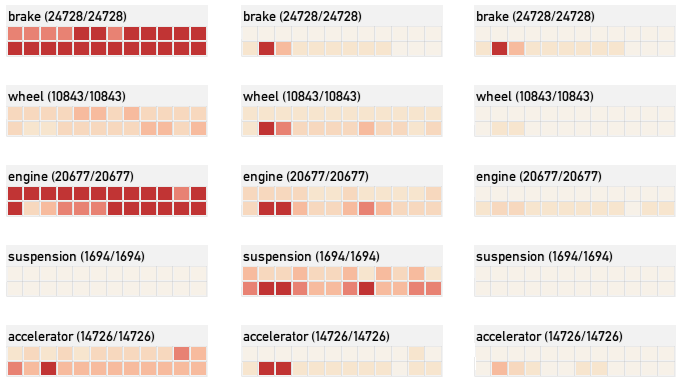
\includegraphics[width=\columnwidth]{heatmap.png}
 \caption{Showing the different heatmap perspectives. Left displays the monthly
 perspective, centre displays the component perspective, and right displays the
 global perspective}
 \label{figure:heatmap}
\end{figure}

\subsection{Comparison}
Comparison mode allows people to compare two different types of the same
physical product specified by two different query sets Q1 and Q2. Every entity
from a query set is matched against the same named entity in the other query
set, producing an entity level based comparison. For example, we can compare how
each car component fared against each other in a comparison of Honda Civic
versus Toyota Corolla, or comparing Ford Focus against the industry form.

Two separate measures are used for the comparison view. A contribution sum and a
percentage difference. The contribution sum is the aggregated entity score from
the two query sets, it reflects the overall importance of the entity by
emphasizing the frequently occurring entities in one or both query set. The
percentage difference describes the relative frequencies of an entity, whether
it occurs more frequently under Q1 or Q2 relative to the total contributions
from Q1 and Q2 respectively. The percentage score is calculated as entity score
divided by the total contribution. Then the percentage difference follows as
percentage score Q1 minus percentage score Q2, with the sign and magnitude
indicating  which query set has the stronger presence. We made the decision to
use percentage based comparisons because it enables as to compare query results
of different sizes.

We encode the sum score as the colour of the \threed component, based on the
default colour scale. For the difference, we render the measure as an outline
around the object. The sign of the difference is encoded as one of two diverging
colours, one for positive and one for negative values. The magnitude of the
difference is encoded as the transparency of the outline, larger magnitude have
more distinct, solid outlines compared to smaller values. Thus, a highly
problematic object from both side will have a strong presence overall but with a
faint outline, while a lopsided but infrequent problem will have strong outline
but barely visible interior colour.

By default, comparison mode is turned off. It is activated when the viewer
switches the second hierarchy filter from the ``None'' position to a valid
selection. Subsequent query modifications are carried out in comparison mode
until the selection is turned to ``None'' again.

One limitation with this approach is our current usage of the total
contributions to calculate the percentage scores. Our total contribution is in
relations to the number of documents in the corpus, which may or may not be a
good indication of the overall contribution. 


%The of the limitation in the current prototype is that we do not have any
%normalization of comparative scores, thus it only makes sense comparing two 
%different types of products with similar volumes.

\subsection{Aggregation}
By default, the system treats each object individually rather than object
groups. For example ``seatbelt'', ``backrest'' and ``seat'' are all scored
separately, even though they are logically under the group ``seat''. This
setting allows people to isolate and identify unique problems accurately. There
are times, however, when this level of information is unnecessarily detailed and
a higher level overview is desirable.

Aggregation mode mimics the type of high level rating system found on consumers
review websites. When aggregation mode is enabled, individual objects, and their
scores are aggregated up to the first level entities. In our specific case, the 
first level are the major sub-systems in a vehicle. The visualization responds
by making all child objects referencing the aggregated score of their parent
subsystem. 

Aggregation mode is enabled/disabled by a toggle switch located at the bottom
left of the user interface. Aggregation mode works in conjunction with
comparison mode, allow people to make comparison of major systems.

\begin{figure}
 \centering  
 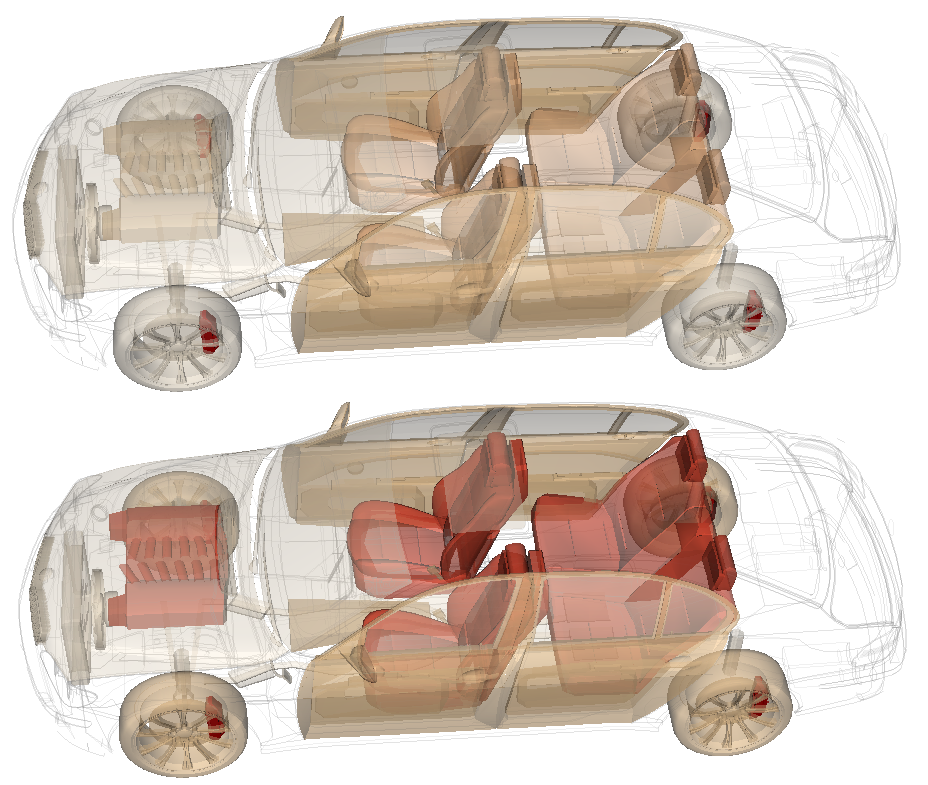
\includegraphics[width=\columnwidth]{aggregation.png}
 \caption{Top: Aggregation mode disabled. Bottom: Aggregation mode enabled,
 note that the seat and engine now appears more prominent in the visualization.}
 \label{figure:heatmap}
\end{figure}
